% Validation section should include: 
% Data/MC Agreement after precuts on all important variables
% Sideband Checks
% Corsika In-time vs BNB-ext
% Future Validation Studies

\section{Validation}
\subsection{Electromagnetic shower energy loss}
A way to verify if we are effectively selecting electron neutrinos is to study the distribution of the electromagnetic showers energy loss per length $dE/dx$. If the data events contain a well-reconstructed electron in the final state, the $dE/dx$ distribution will be peaked around 2~MeV/cm.
Figure \ref{fig:dedx_after} shows the $dE/dx$ distributions for data and Monte Carlo after the application of the rectangular cuts (left) and after the application of the BDTs cuts (right). As expected, the peak is in both cases around 2~MeV/cm, meaning that the $dE/dx$ of the reconstructed showers in data are compatible with electrons in the final state.

\begin{figure}[htbp]
\centering
  \begin{subfigure}{0.48\textwidth}
    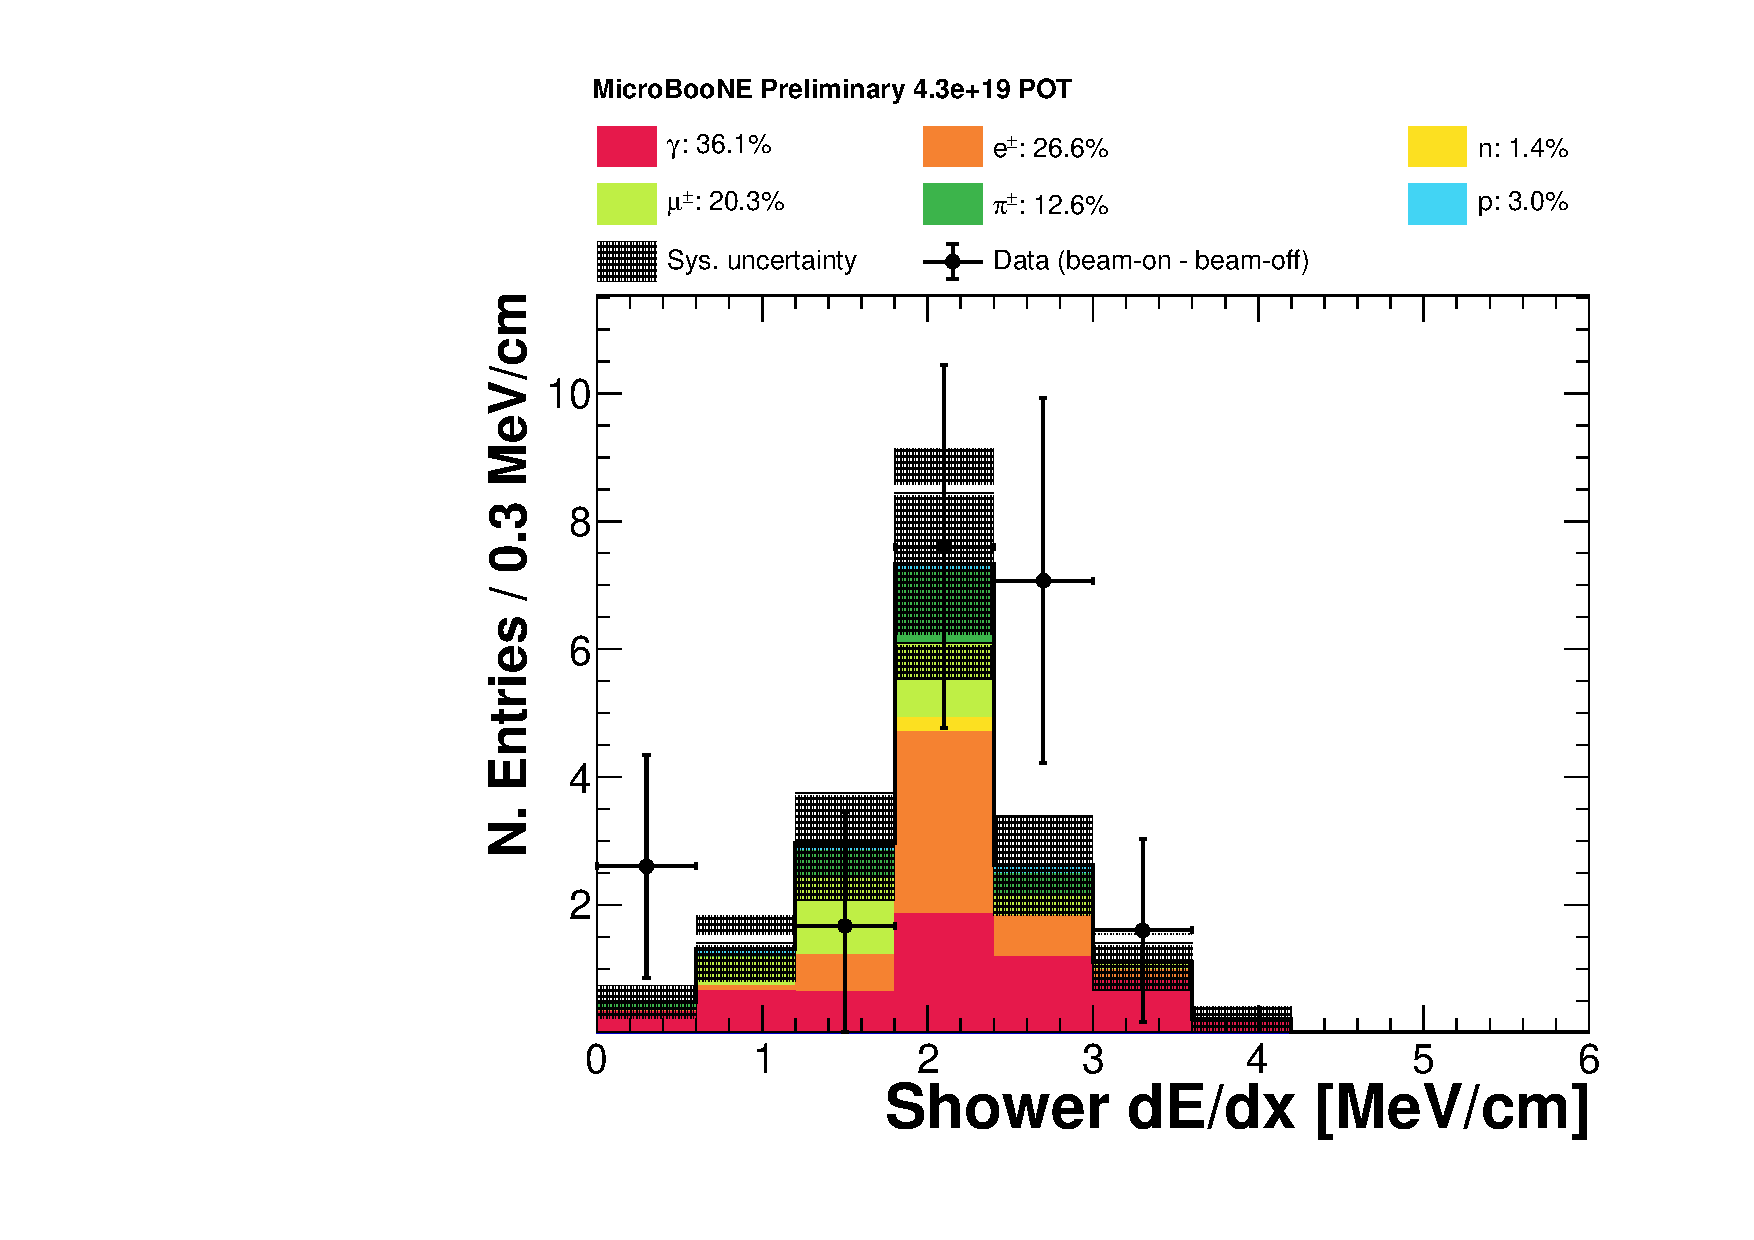
\includegraphics[width=\linewidth]{figures/dedx_cuts.pdf}
    \caption{Rectangular cuts.} 
  \end{subfigure}
    \begin{subfigure}{0.48\textwidth}
    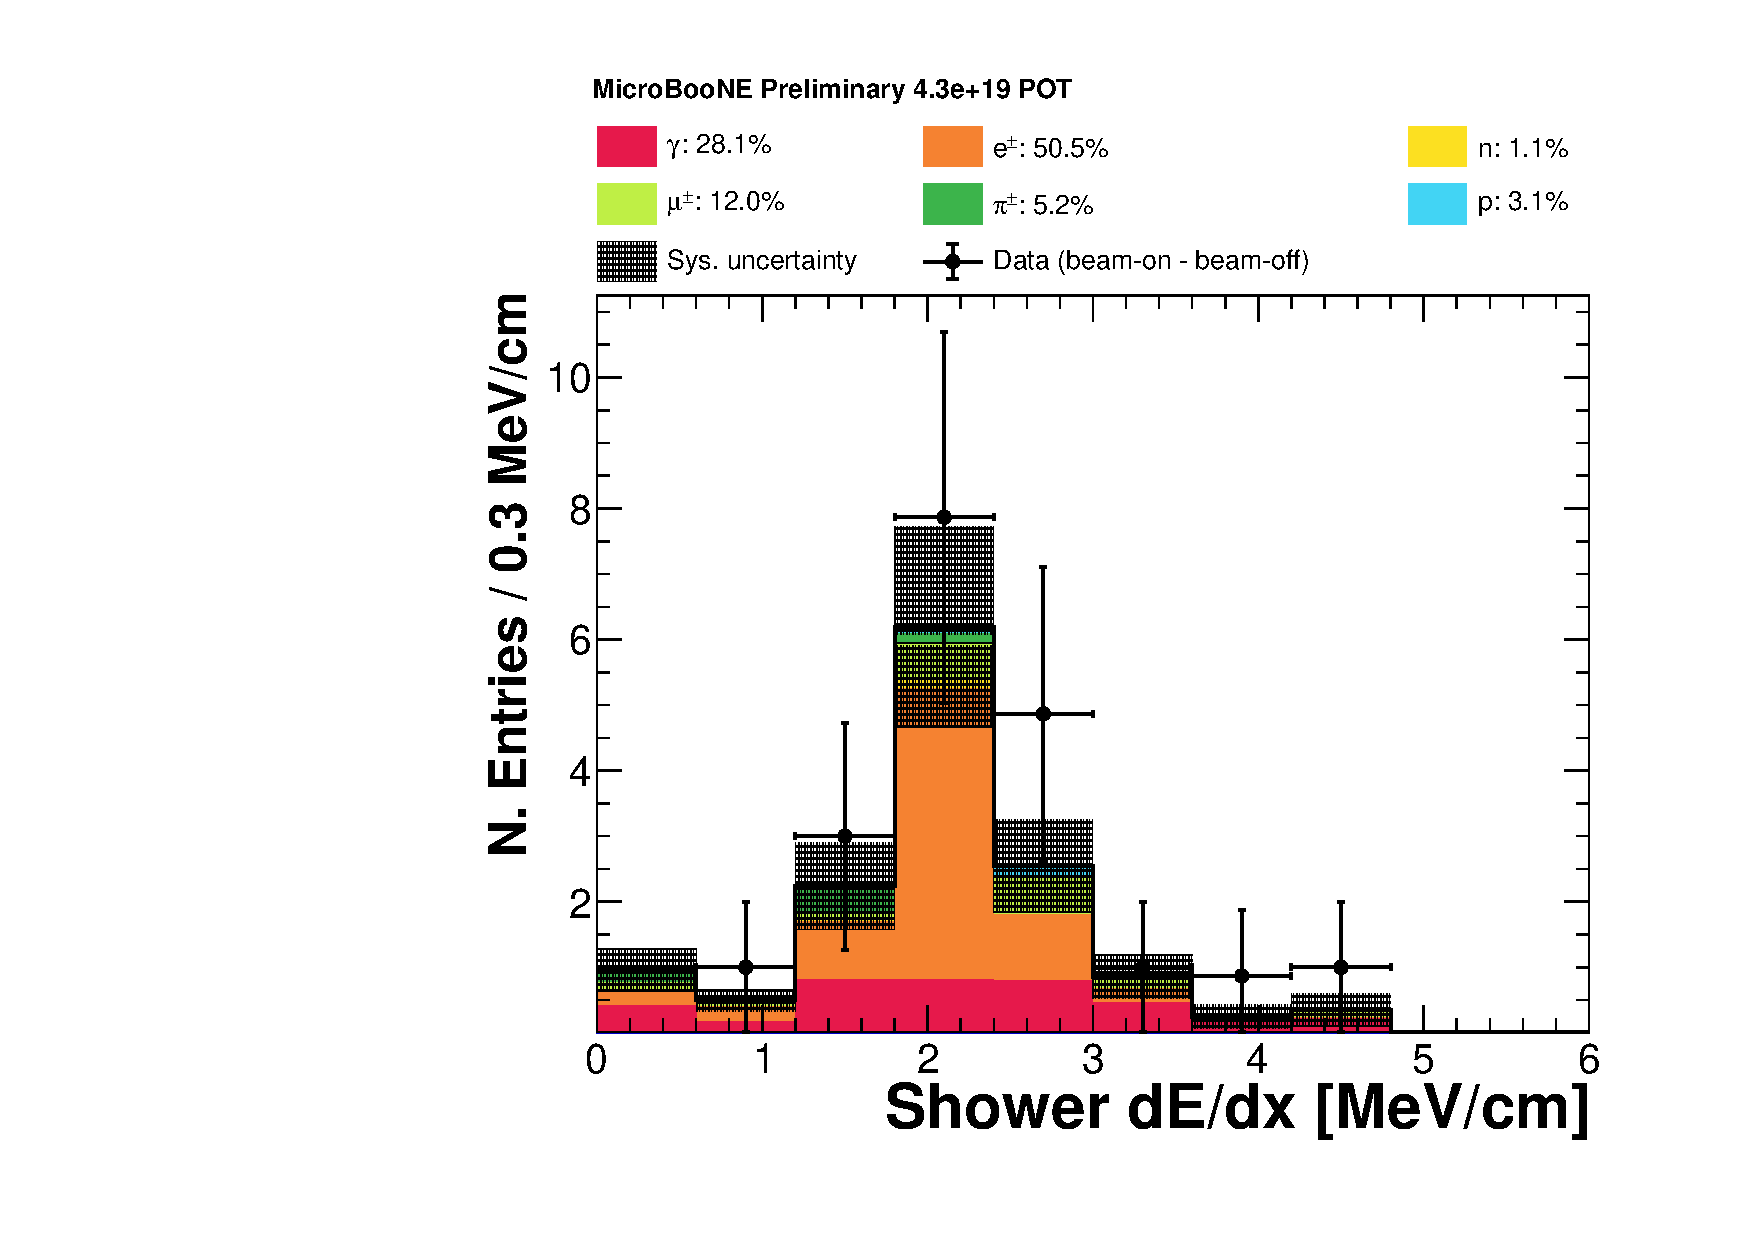
\includegraphics[width=\linewidth]{figures/dedx_bdt.pdf}
    \caption{BDTs.} 
  \end{subfigure}
  \caption{Distribution of the reconstructed showers $dE/dx$ after rectangular cuts (left) and BDTs cuts (right).}
  \label{fig:dedx_after}
\end{figure}

\subsection{Side-bands checks}
In this section we will study the agreement between data and Monte Carlo for selected samples orthogonal to our $\nu_{e}$ CC0$\pi$-Np signal. In order to validate our analysis, some of the background cuts described in Section \ref{sec:bkg} are inverted or removed in order to enhance different background components.
\subsubsection{Photon-enhanced selection}
It is possible to enhance the neutral-current component (defined as \emph{beam intrinsic NC} in our analysis) by (1) inverting the cut on the shower $dE/dx$, , and (2) removing the cut on the shower distance (see Figures \ref{fig:dedx_norm}, \ref{fig:showerd_norm}). The $dE/dx$ of the most energetic shower must be within 3.2~MeV/cm and 5~MeV/cm to select electromagnetic cascades that were initiated by a photon. It also ensures that this photon-enhanced sample is orthogonal to the $\nu_{e}$ CC0$\pi$-Np selected sample. The cut on the shower distance is removed to include events where the photon conversion is far from the neutrino interaction vertex.
Thus, our final sample will mainly contain NC events, with some contamination of $\nu_{\mu}$ CC$\pi^{0}$ events where the muon track was tagged as a proton-like track.

Figure \ref{fig:photon} shows the comparison between data and Monte Carlo for the reconstructed energy spectrum $E_{deposited}$ of the photon-enhanced event spectrum. 
%The reconstructed energy $E_{corr}$ here corresponds to the sum of the reconstructed energies of the shower-like objects and the reconstructed energies of the track-like objects $E_{corr} = E_{corr}^{p}+E_{corr}^{e}$.

\begin{figure}[htbp]
\centering
  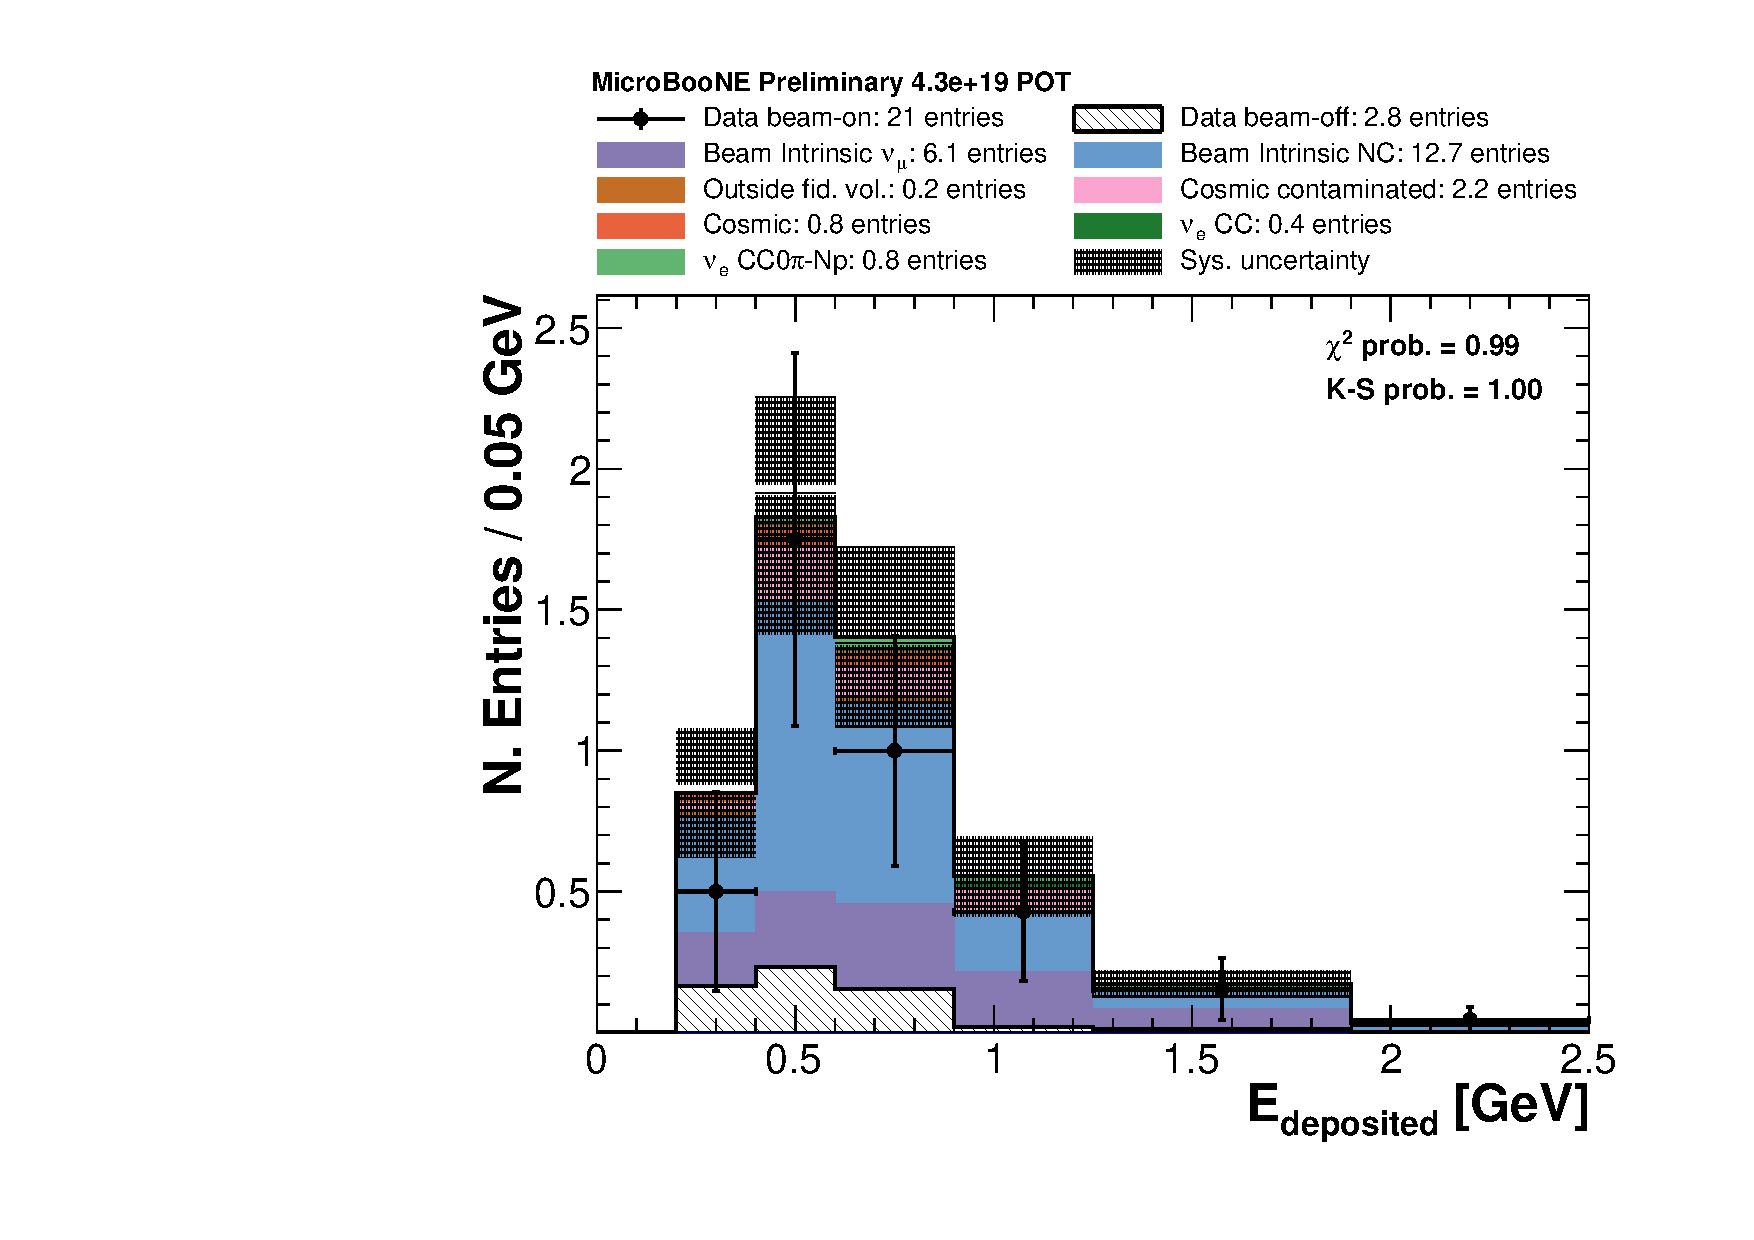
\includegraphics[width=0.7\linewidth]{figures/nc_reco.pdf}
  \caption{Reconstructed energy spectrum of the events selected with the photon-enhanced reverse cuts.}\label{fig:photon}
\end{figure}

\subsubsection{CC \texorpdfstring{$\nu_{\mu}$}{numu}-enhanced reverse cuts}
It is possible to enhance the presence of the CC $\nu_{\mu}$ background (defined as \emph{beam intrinsic $\nu_{\mu}$} in our analysis) by (1) removing the cut on the total number of hits in the collection plane, (2) removing the cut on the fraction of shower hits, (3) requiring a minimum track length, (4) requiring at least a track with $40 < \chi_p^{2} < 220$ (muon-like track), and (5) requiring that the event is selected by the external $\nu_{\mu}$ CC-inclusive analysis \cite{ubxsec} (see Figures \ref{fig:proton_norm}, \ref{fig:length_norm}). Also in this case the CC $\nu_{\mu}$-enhanced sample will be orthogonal to the $\nu_{e}$ CC0$\pi$-Np selected sample.
A CC $\nu_{\mu}$ event has, by definition, a muon in the final state: as such, requiring a track length larger than 20~cm and changing the cut on the proton $\chi^2_p$ score decreases our muon-rejection power. The goal of the external analysis is to select CC $\nu_{\mu}$ events, so instead of vetoing those events as described in Section \ref{sec:numu}, we invert this requirement by allowing only these events.

Figure \ref{fig:numu_inverted} shows the agreement between data and Monte Carlo for the reconstructed energy spectrum of the CC $\nu_{\mu}$-enhanced event spectrum.

\begin{figure}[htbp]
\centering
  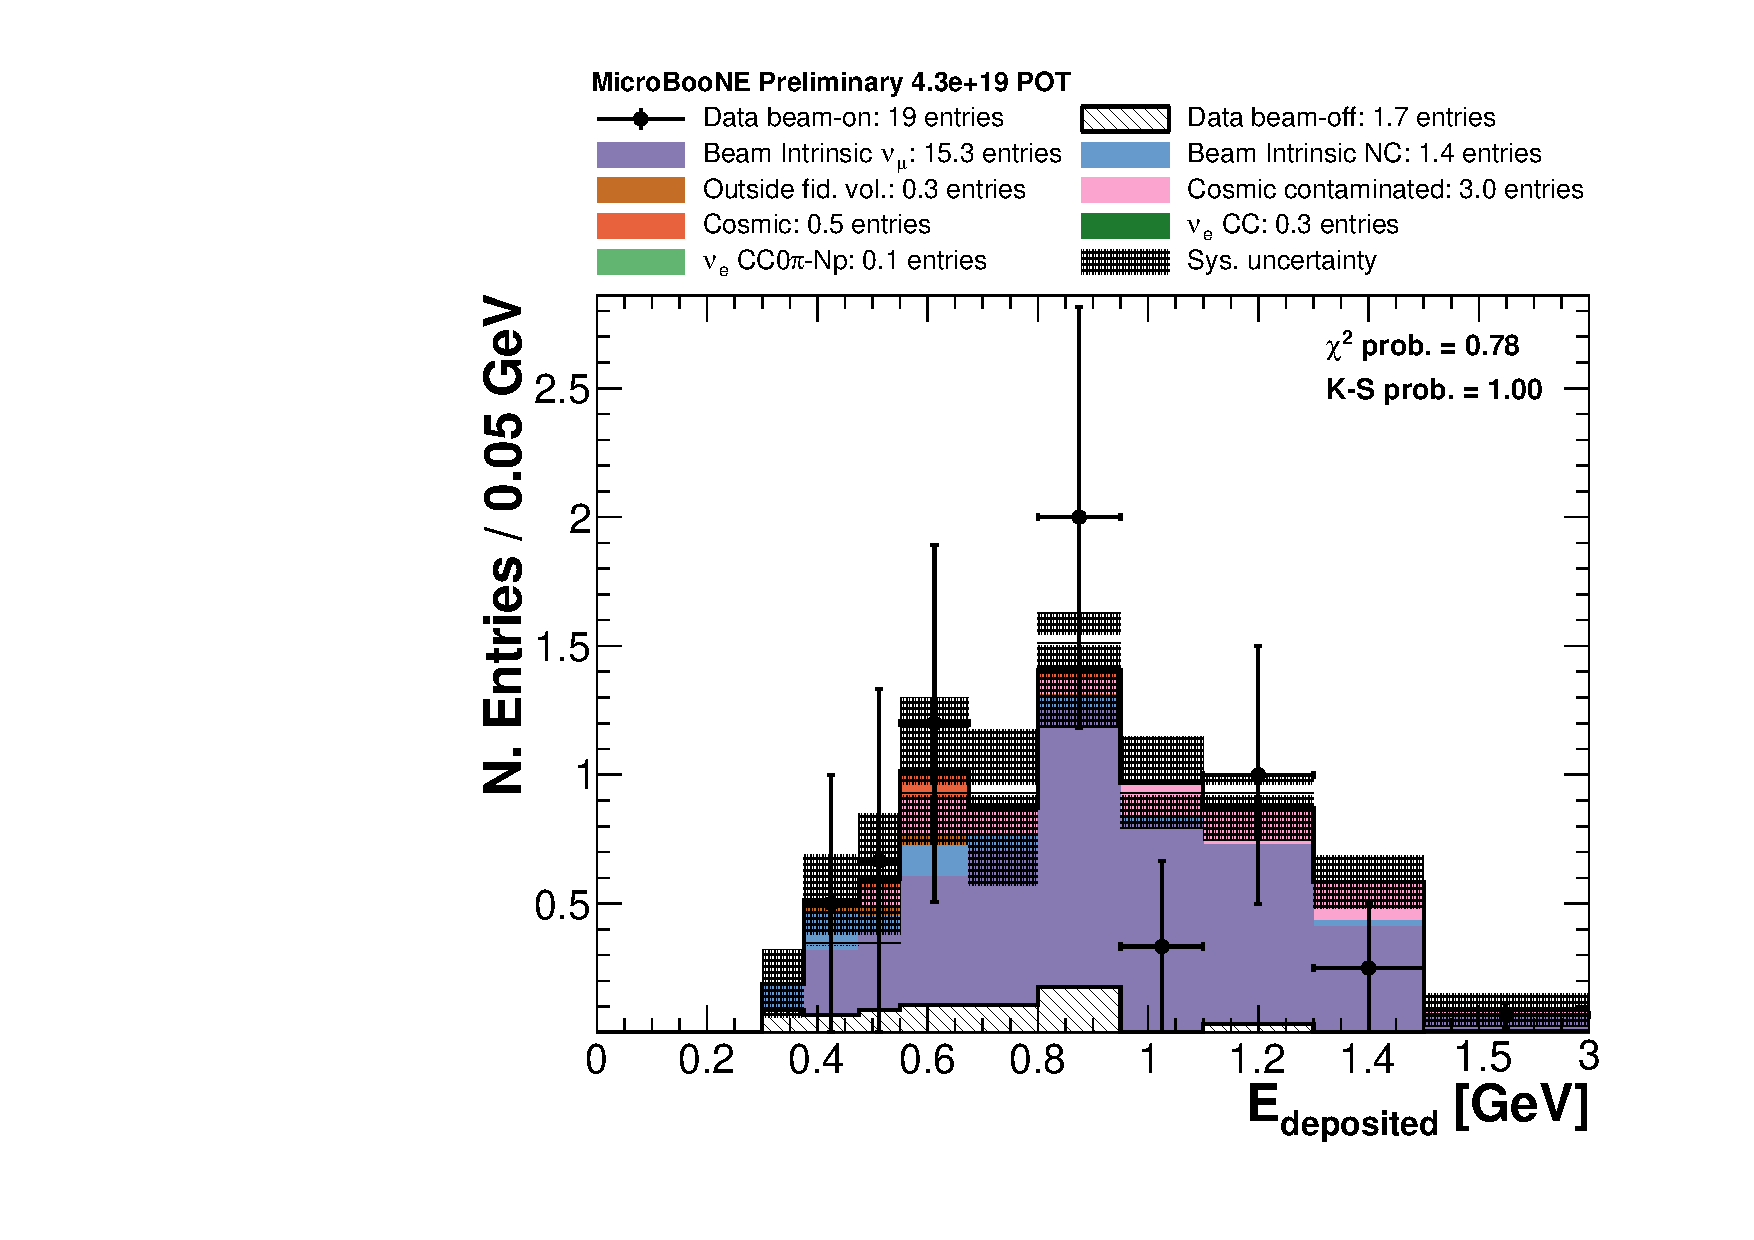
\includegraphics[width=0.7\linewidth]{figures/numu_reco.pdf}
  \caption{Reconstructed energy spectrum of the events selected with the CC $\nu_{\mu}$-enhanced reverse cuts.}\label{fig:numu_inverted}
\end{figure}

% \subsection{Future Validation Studies}

% \subsubsection{Cosmic-ray studies}
% In order to validate the cosmic-ray components of our selected events it is possible to compare simulated events with a CORSIKA cosmic ray producing a flash in the optical system during the beam-gate window and the data off-beam sample. 
% In this way we will be able to check if the distributions of the variables we use (e.g. shower energy, shower $dE/dx$) show a good agreement between the simulation and a well-understood set of data events. 
% It will help to validate the cosmic background components and also the energy and $dE/dx$ reconstruction procedures.

\subsection{NuMI beam event studies}
It is possible to run this analysis on the complementary NuMI dataset, acquired with the NuMI beam trigger. The NuMI beam is created from 120 GeV protons hitting a carbon target \cite{Adamson:2015dkw}, while the BNB is created from 8 GeV protons on a beryllium target. The NuMI beam has also a higher intrinsic $\nu_{e}$ component than the BNB (5\% vs. 0.5\%). Figure \ref{fig:numibeam} shows a comparison of the NuMI and BNB beam fluxes for the MicroBooNE detector. Even though it is around $8^{\circ}$ off-axis, MicroBooNE still receives $\sim2500$ $\nu_{e}$ interactions per year. 

As such, a study of the events selected in the NuMI dataset is of fundamental importance to validate the $\nu_{e}$ CC0$\pi$-Np selection algorithm, since it provides a completely independent set of electron neutrinos with different energy and angular distributions.

\begin{figure}[htbp]
\centering
  \begin{subfigure}{0.45\textwidth}
    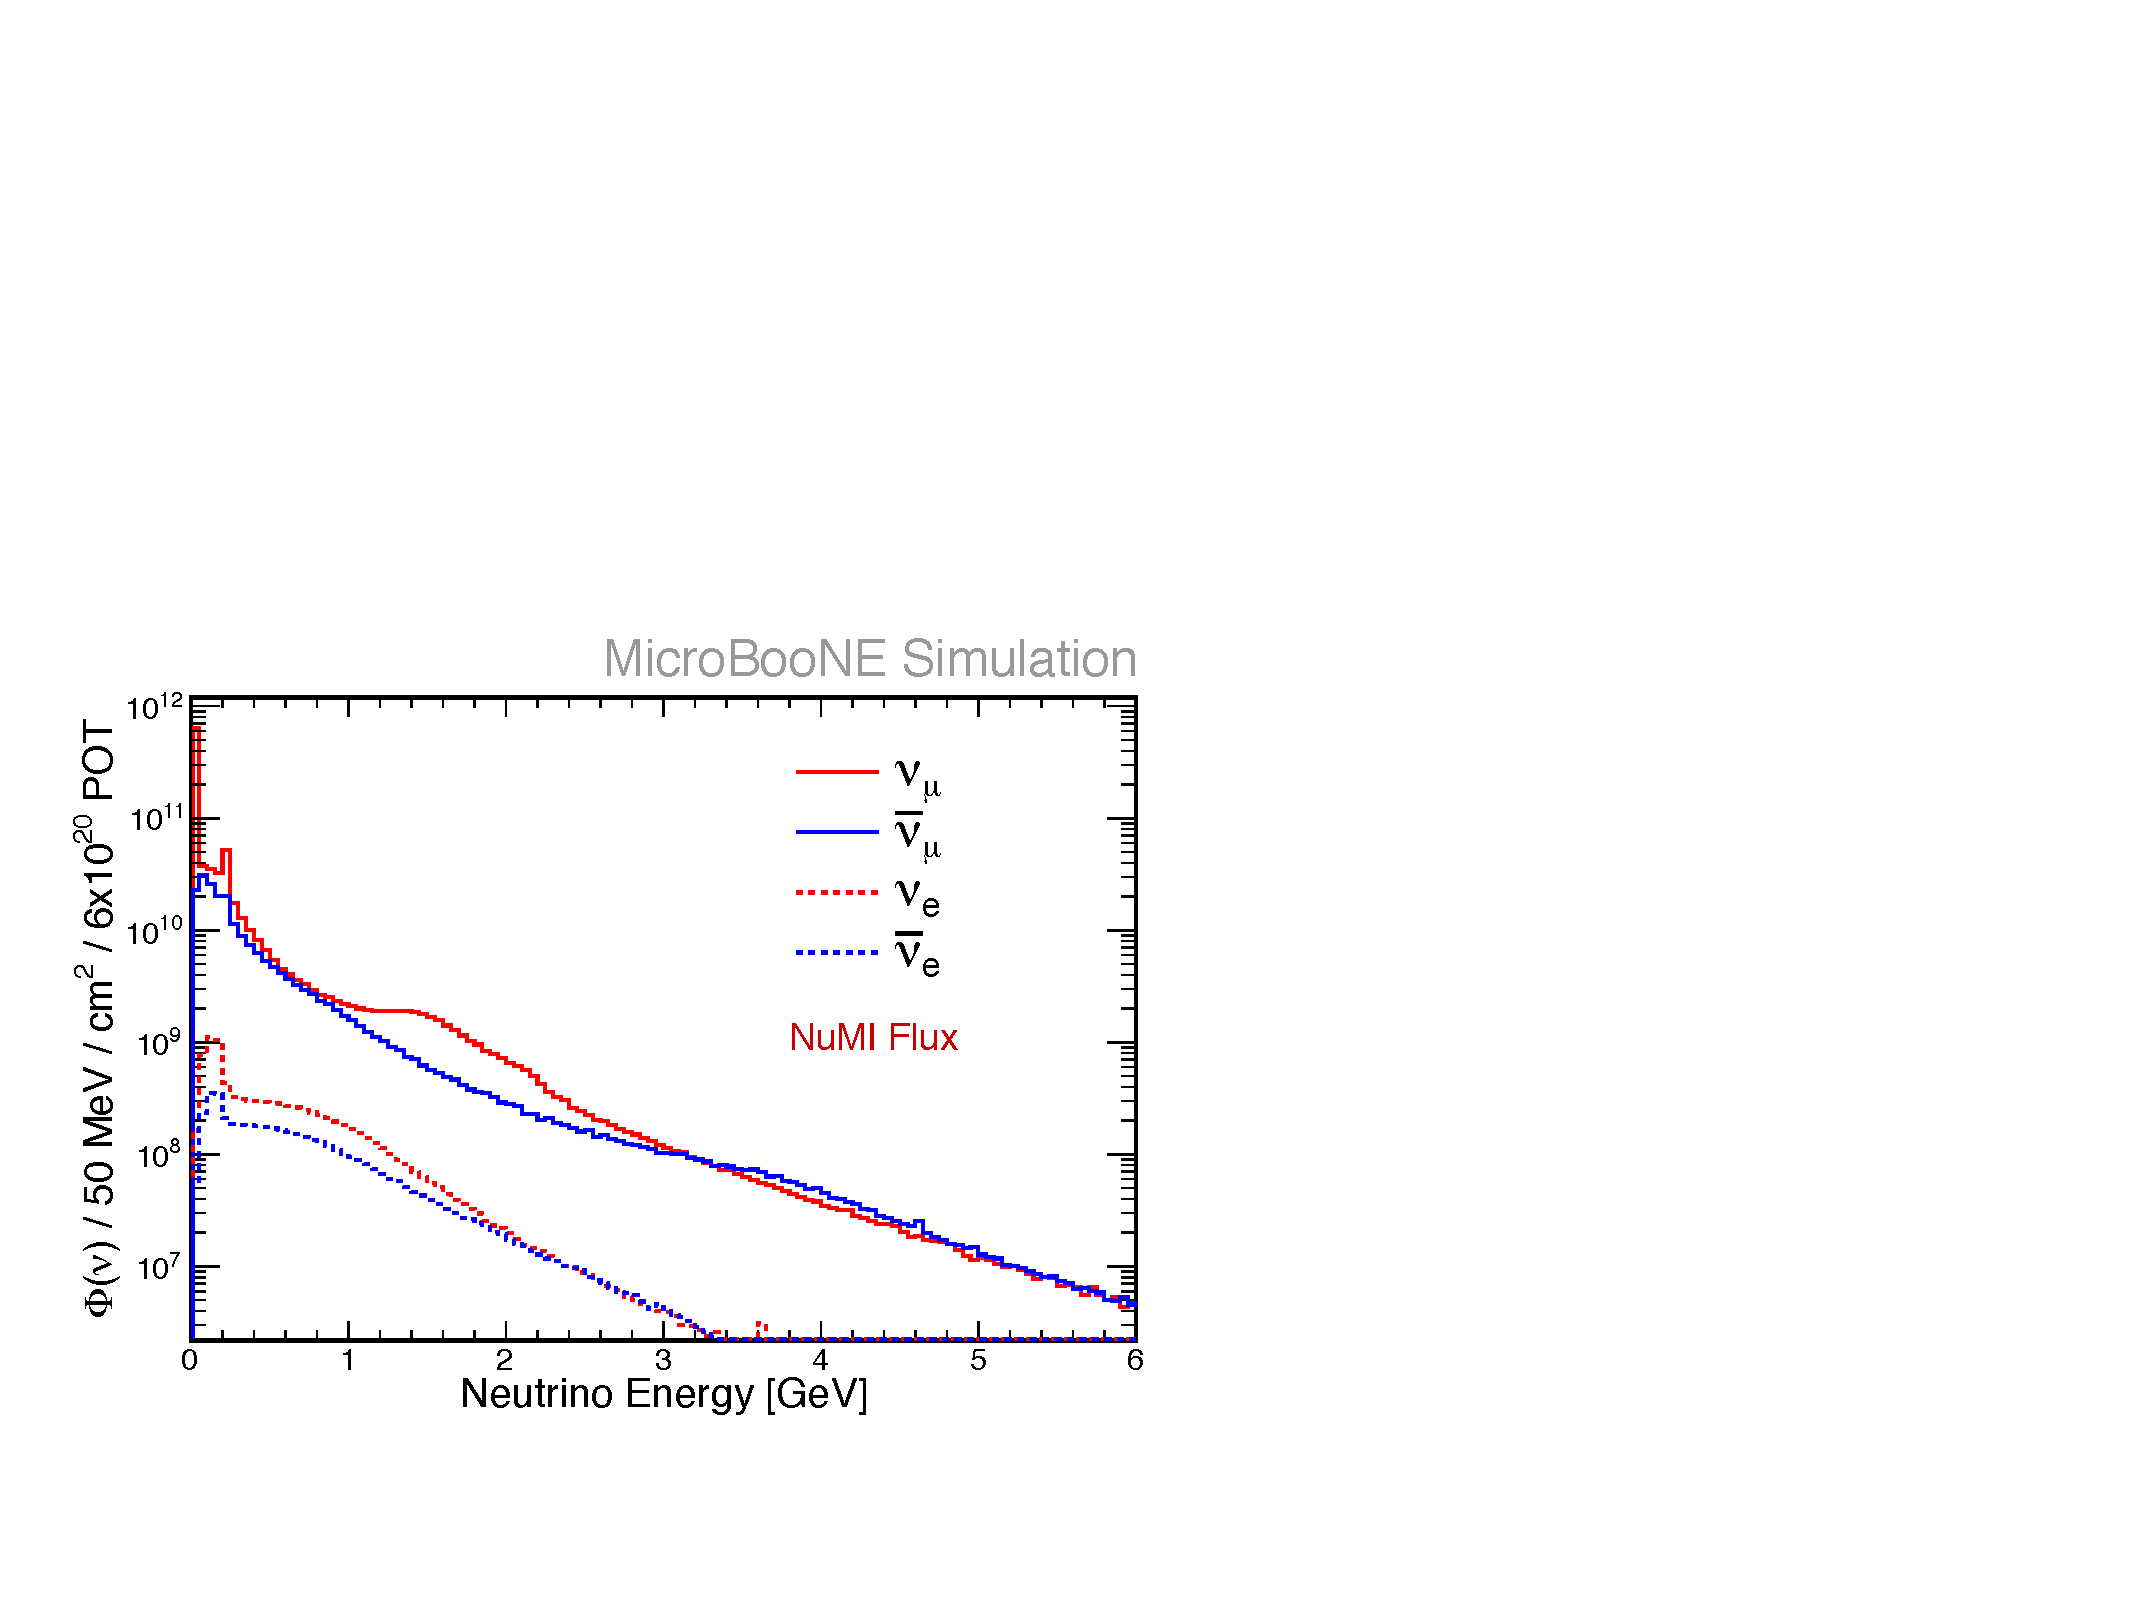
\includegraphics[width=\linewidth]{figures/numi.pdf}
    \caption{NuMI beam flux.} 
  \end{subfigure}
    \begin{subfigure}{0.45\textwidth}
    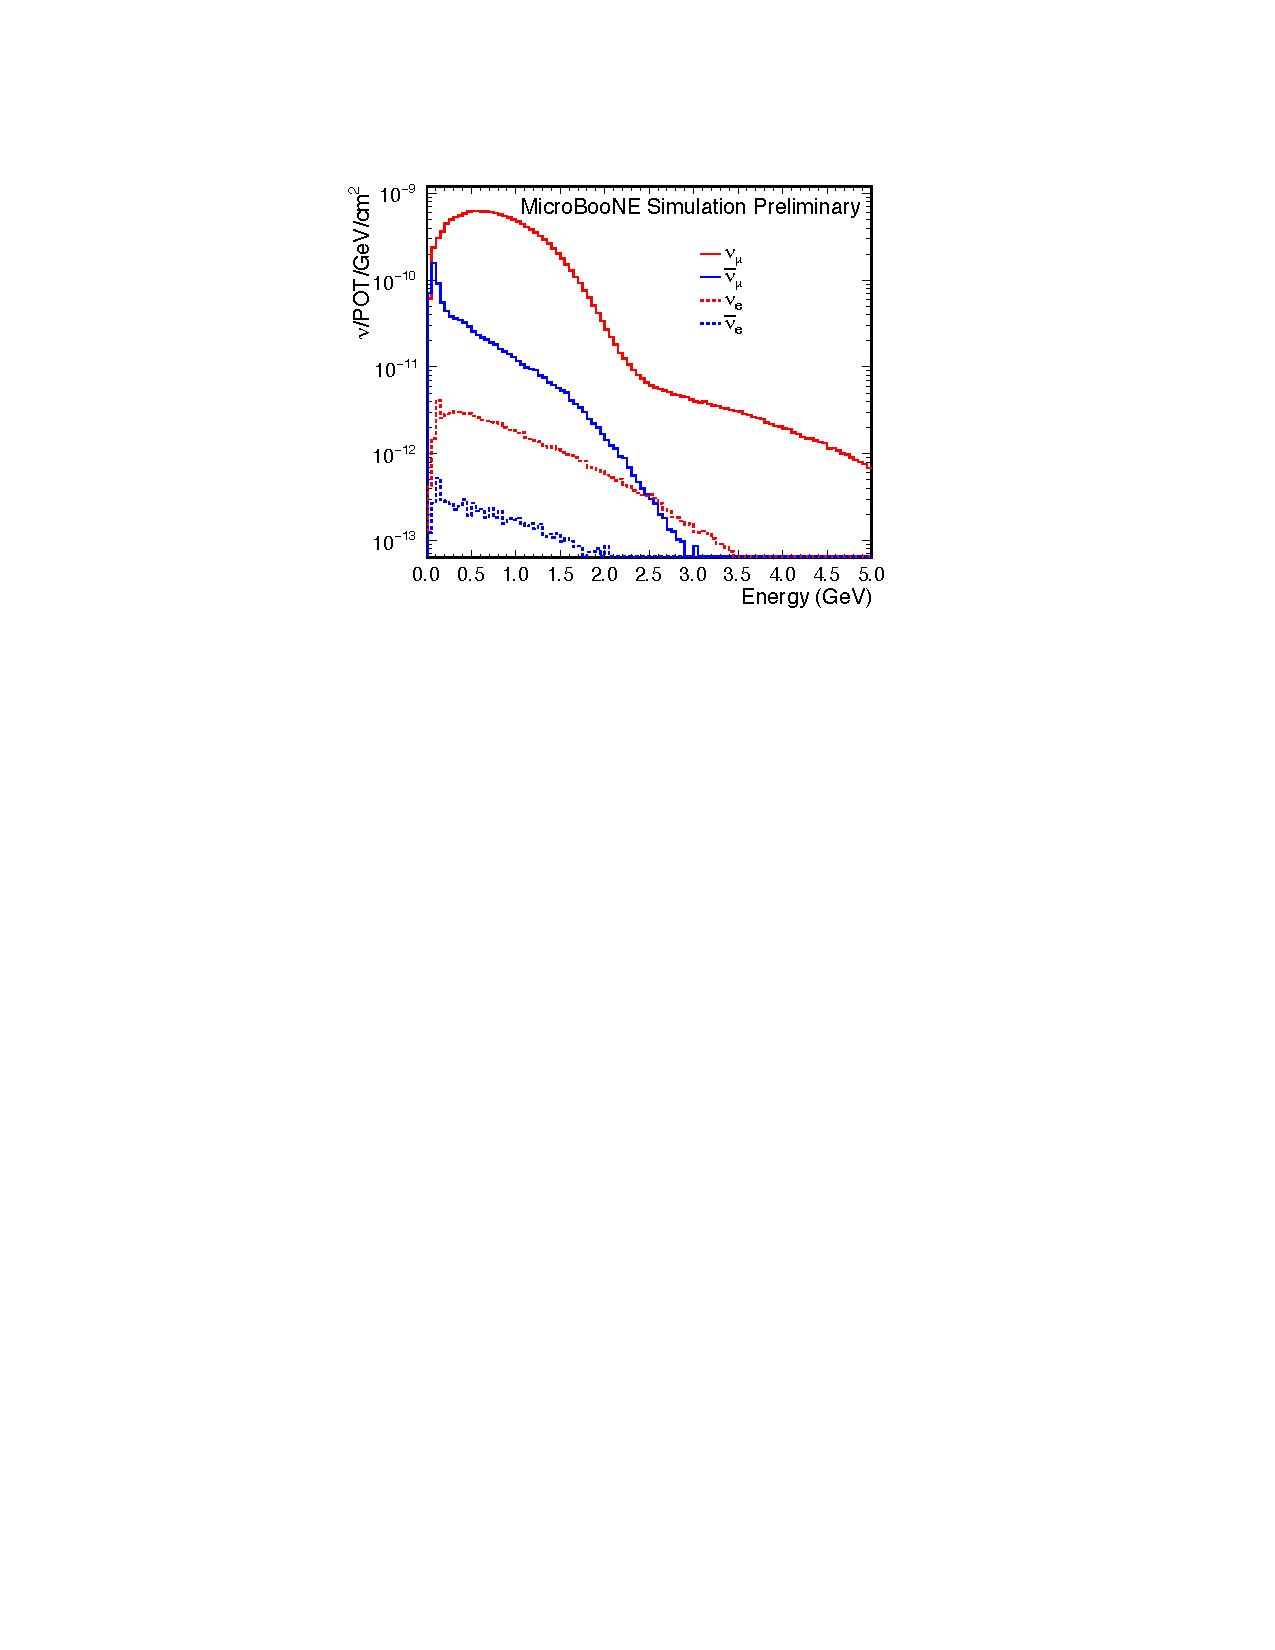
\includegraphics[width=\linewidth]{figures/bnbflux.pdf}
    \caption{BNB beam flux.} 
  \end{subfigure}
  \caption{NuMI and BNB neutrino fluxes for each neutrino and antineutrino component, when the beams are in neutrino mode.}\label{fig:numibeam}
\end{figure}

In order to run on this data sample, it is necessary to change the requirement on the reconstructed flash, since the beam-gate window is $[6,16]$~\si{\micro}s after the trigger time.
We apply the same rectangular cuts described in Section \ref{sec:cuts}, plus a threshold of 100~MeV on the reconstructed energy of the leading shower. This last cut allows us to remove a large fraction of cosmogenic background without significantly affecting our $\nu_e$ CC0$\pi$-Np selection efficiency, since the NuMI beam has a higher energy than the BNB.

\begin{figure}[htbp]
\centering
  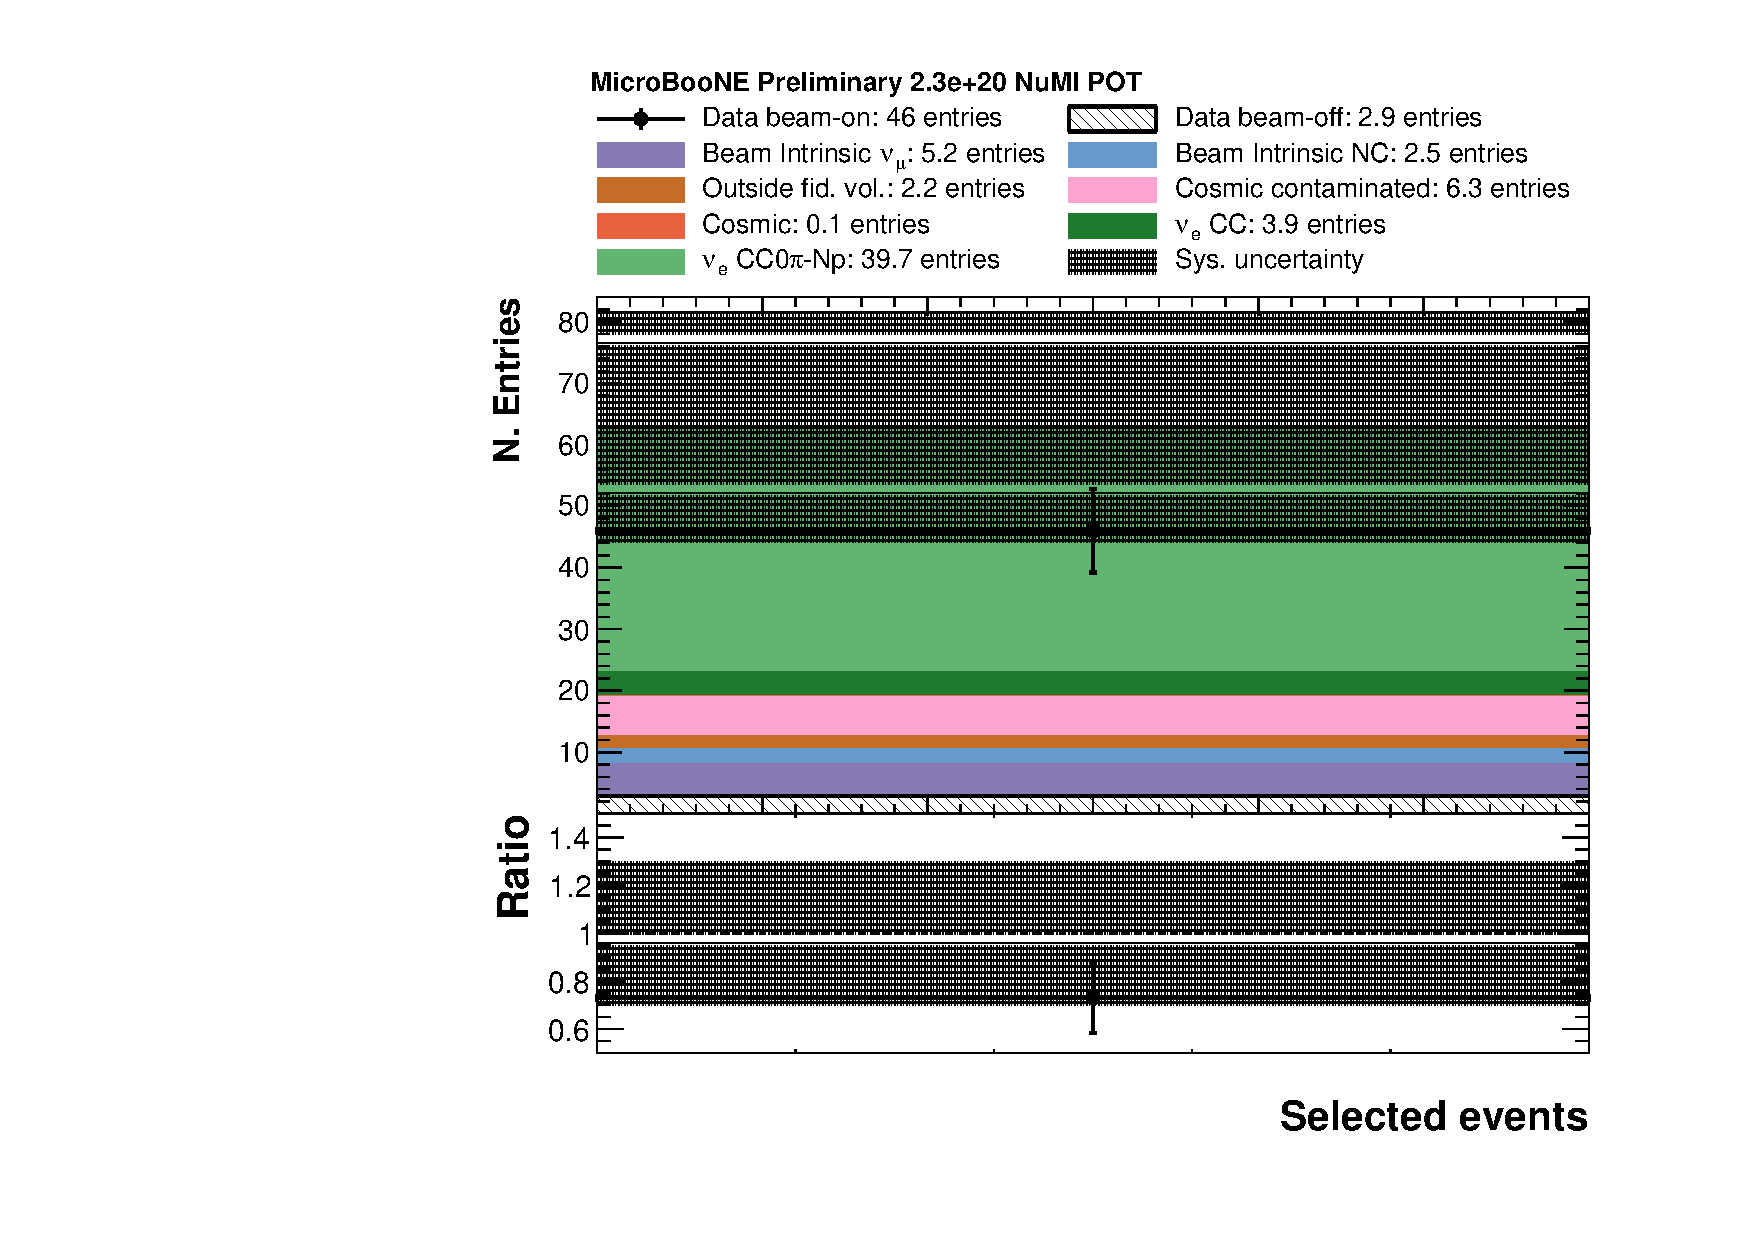
\includegraphics[width=0.75\linewidth]{figures/numi_events.pdf}
  \caption{Number of selected events after selection and rectangular cuts, classified according to the event category and corresponding to an exposure of $2.3\times10^{20}$ NuMI POT in neutrino mode.}\label{fig:numi_nue}
\end{figure}

Figure \ref{fig:numi_nue} shows the number of selected events in data and Monte Carlo for $2.3\times10^{20}$ NuMI POT, collected between February and June 2016 in neutrino mode. Proper systematic uncertainties for NuMI events still need to be assessed, since the off-axis positioning introduces a large uncertainty in the flux that needs to be carefully evaluated. A conservative estimate gives an expected 30\% systematic uncertainty in the number of selected events.

We select 46 data events, 39.7 signal ($\nu_e$~CC0$\pi$-Np) events, and 23.1 background events. In order to calculate the significance of the detection of $\nu_e$~CC0$\pi$-Np events, it is necessary to take into account the large size of the signal $s$ with respect to the background $b$. In this case, the usual formula:
\begin{equation}
    \sigma = \frac{s}{\sqrt{b}}
\end{equation}
is not valid. Thus, we adopt a profile-likelihood ratio test, as described in \cite{Cowan:2010js}.
Assuming a 30\% systematic uncertainty, the expected (observed) significance for the detection of $\nu_e$~CC0$\pi$-Np events is 3.4$\sigma$ (2.2$\sigma$). The statistical-only significance is $6.8\sigma$ ($4.2\sigma$).

